%%%%%%%%%%%%%%%%%%%%%%%%%%%%%%%%%%%%%%%%%%%%%%%%%%%%%%%%%%%%%%%%%%
%%%%%%%%%%%%%%%%%%%%%%%%%%%%%%%%%%%%%%%%%%%%%%%%%%%%%%%%%%%%%%%%%%
%% FRAME-FILE
%%
%% Author        : Stefan M. Moser,
%%
%% Written       : January 1998, based on a file by Michael Semling
%%
%% Modifications : ongoing, used for semester project 1, semester
%%                 project 2, master thesis, PPS, SADA @ ISI
%%
%% Last Modify.   : 21 May 2004, 24 Oct 2006 (Michèle Wigger)
%%
%% Version       : 3.4
%%
%% Copyright     : Free for distribution if 
%%                     - you keep this header (you may add to it!)
%%                     - you do not charge any fee
%%
%%%%%%%%%%%%%%%%%%%%%%%%%%%%%%%%%%%%%%%%%%%%%%%%%%%%%%%%%%%%%%%%%%
%%%%%%%%%%%%%%%%%%%%%%%%%%%%%%%%%%%%%%%%%%%%%%%%%%%%%%%%%%%%%%%%%%
%% HELP:
%%
%% Compilation of file:
%%
%%  latex frame; bibtex frame; latex frame; latex frame
%%
%%  dvips -Pcmz -Pamz -Psuper -o frame.ps frame.dvi
%% 
%%
%%%%%%%%%%%%%%%%%%%%%%%%%%%%%%%%%%%%%%%%%%%%%%%%%%%%%%%%%%%%%%%%%%
%%%%%%%%%%%%%%%%%%%%%%%%%%%%%%%%%%%%%%%%%%%%%%%%%%%%%%%%%%%%%%%%%%
%% HELP ONLINE:
%%
%% http://computing.ee.ethz.ch/.soft/latex/tetex/     (tardis)
%%
%% file:/usr/pack/tetex-1.0.7-mo/texmf/doc/index.html (ISI)
%%
%% CTAN for any package: http://www.ucc.ie/cgi-bin/ctan
%%
%%%%%%%%%%%%%%%%%%%%%%%%%%%%%%%%%%%%%%%%%%%%%%%%%%%%%%%%%%%%%%%%%%
%%%%%%%%%%%%%%%%%%%%%%%%%%%%%%%%%%%%%%%%%%%%%%%%%%%%%%%%%%%%%%%%%%
%% Styles: article, book, report
\documentclass[11pt,a4paper,twoside]{report}
\pdfoutput=1
%
%% Draft:
%
%\documentclass[draft,11pt,a4paper,twoside,dvips]{report}
                                    % On border a black ruler shows
                                    % lines with problems
%\usepackage[notref, notcite]{showkeys}
                                    % All labels are printed on the
                                    % side 
%
%%%%%%%%%%%%%%%%%%%%%%%%%%%%%%%%%%%%%%%%%%%%%%%%%%%%%%%%%%%%%%%%%%
%% PACKAGES                         DESCRIPTION
%%%%%%%%%%%%%%%%%%%%%%%%%%%%%%%%%%%%%%%%%%%%%%%%%%%%%%%%%%%%%%%%%%
\usepackage[ngerman,USenglish]{babel} % Different languages:
                                    % Swap between the languages
                                    % with \selectlanguage{sprache} 
%\usepackage[latin1]{inputenc}      % acceptance of german Umlaute


%\usepackage{bibtex/macros}  %for IEEE transaction submission it is not allowed to have a separate style-file :-( :-( :-(
\usepackage{blindtext}
\usepackage{etex}				%mehr register etc.
\usepackage{algorithmicx}
\usepackage{times}
%\usepackage{psfrag}
\usepackage{graphicx}
\usepackage{graphics}
%\usepackage{pstricks,pst-node,pst-tree}
\usepackage{epsfig}
\usepackage{amssymb}
\usepackage{amsmath}
\usepackage{amsthm}
\usepackage{color}
\usepackage{fancyhdr}
%\PassOptionsToPackage{hyphens}{url}

%Raban: Added Joe's style
\usepackage[bookmarks,colorlinks,breaklinks]{hyperref}  % PDF hyperlinks, with coloured links
\definecolor{dullmagenta}{rgb}{0.4,0,0.4}   % #660066
\definecolor{darkblue}{rgb}{0,0,0.4}
\hypersetup{linkcolor=red,citecolor=blue,filecolor=dullmagenta,urlcolor=darkblue} % coloured links



%\usepackage[colorlinks,urlcolor=blue] {hyperref}    %change here colorlinks=false to remove the colored links (for print-version)
\usepackage{url}
%\usepackage[colorlinks, hyperindex,pagebackref] {hyperref}
%\usepackage{backref}
\urlstyle{tt}


%zusaetzlich nicht standard
%\usepackage{amsfonts}		%mathematisches Menge R, N
%\usepackage{mathrsfs}
%\usepackage[usenames]{color}
%\usepackage{textcomp}
%\usepackage{latexsym}		%f�r Re(z) und Img(z)
%\usepackage{amsthm}
%\usepackage{wrapfig}
%\usepackage{pdfpages}
%\usepackage{caption}
%\usepackage{subfig}
\usepackage{listings}

%fuer TikZ zum Zeichnen von Graphiken
\usepackage{tikz}
\usetikzlibrary{chains}
\usetikzlibrary{fit}
\usepackage{pgflibraryarrows}		%optional
\usepackage{pgflibrarysnakes}		%optional
\usepackage{epsfig}

% Added by Raban
\usepackage{enumerate}  
\usepackage{nicefrac} 
\usepackage{braket}
\usepackage{caption}
\usepackage{subcaption}

\usepackage{bm}  % Define \bm{} to use bold math fonts
\usepackage{bbm}
\usepackage{xcolor}
\usepackage{verbatim}
\usepackage{natbib}
\makeatletter
\makeatother

\begin{comment}
%-------------- start insert modified commands ------------------
\makeatletter
\def\blx@bblfile@bibtex{%
 \blx@secinit
 \begingroup
 \blx@bblstart
%%%%%%%%%%%%%%%%%%%%%%%%%%%%%%%%%%%%%
%
\input{biblio_MA.bbl}
%
%%%%%%%%%%%%%%%%%%%%%%%%%%%%%%%%%%%%%
 \blx@bblend
 \endgroup
 \csnumgdef{blx@labelnumber@\the\c@refsection}{0}}
\makeatother
%-------------- end insert modified commands ------------------
\end{comment}


%\usetikzlibrary{external}
%\usetikzlibrary{decorations.pathreplacing}
%\tikzexternalize[prefix=ConfPaper-]


%\include{psfig}

\usepackage{listings}
\usepackage{url}

\usepackage{algorithm}
\usepackage[noend]{algpseudocode}


\usepackage[latin1]{inputenc}

\usepackage{paralist} % for enumerate

\usepackage{mathabx} % for nice math symbols
%\usepackage{MnSymbol} % for nice math symbols

\usepackage{footmisc} % for \footref



%%%%%%%%%%%%%%%%%%%%%%%%%%%%%%%%%%%%%%%%%%%%%%%%%%%%%%%%%%%%%%%%%%
%% Macros:
%%%%%%%%%%%%%%%%%%%%%%%%%%%%%%%%%%%%%%%%%%%%%%%%%%%%%%%%%%%%%%%%%%
%% for IEEE transaction submission it is not allowed to have a separate style-file. Therefore we have to copy the commands we used
\def\Hb{\ensuremath{H_{\rm b}}}
\def\S{\mathsf{S}}
\def\D{\mathsf{D}}
\def\C{\mathsf{C}}
\def\T{\mathsf{T}}
\def\E{\mathsf{E}}
\def\F{\mathsf{F}}
\def\R{\mathsf{R}}
\def\Z{\mathsf{Z}}
\DeclareMathOperator{\dec}{dec}
\DeclareMathOperator{\decp}{dec'}
\def\Rset{\mathcal{R}_\epsilon}
\def\Dset{\mathcal{D}_\epsilon}
\def\Bparam{Bhattacharyya parameter}

\DeclareMathOperator*{\argmax}{arg\,max}

% Comments
\newcommand{\RI}[1]{{\color[RGB]{0,128,0} *~*~*~ #1 *~*~*~}}

% QRM notaion
\newcommand{\ketbra}[1]{|#1\rangle\langle #1|}
\newcommand{\cnot}{{\footnotesize \textnormal{CNOT}} }
\newcommand{\RM}{\mathcal{RM} }
\newcommand{\QRM}{\mathcal{QRM} }

\newcommand*{\ee}{\mathrm{e}}


%\DeclareMathOperator{\T}{T}
\DeclareMathOperator{\enc}{enc}
\DeclareMathOperator{\EC}{EC}
\def\A{\mathsf{A}}
\def\H{H}
\def\P{P}
\newcommand{\+}{\textnormal{+} }
\newcommand{\bp}{\textbf{+} }
\newcommand{\g}{\hspace{1mm}}
\renewcommand{\d}{\textnormal{d}} %for integration measure
\newcommand{\id}{\textnormal{id}}
\def \I{\mathrm{i}}

% Joe notaion
\def\tr{{\rm tr}}
\def\pr{{\rm Pr}}
\def\Re{{\rm Re}}
\def\cl{{\text{cl}}}
\def\ker{{\text{ker}}}
\def\fpg{F_{{\rm pg}}}
\def\cC{\mathcal C}
\def\cD{\mathcal D}
\def\cE{\mathcal E}
\def\spec{\text{spec}}


\newcommand{\norm}[1]{\left\lVert#1\right\rVert}
\newcommand{\normT}[1]{\left\vert\kern-0.25ex\left\vert\kern-0.25ex\left\vert #1 
    \right\vert\kern-0.25ex\right\vert\kern-0.25ex\right\vert}

% correct bad hyphenation here
\hyphenation{op-tical net-works semi-conduc-tor Spe-ci-fi-cally di-mensio-nal}
\hyphenation{va-rie-ty}
\hyphenation{the-sis}
\hyphenation{opti-ma-li-ty}
\hyphenation{dif-fe-rent}
\hyphenation{ma-the-ma-ti-cal}
\hyphenation{pa-ra-me-ter}
\hyphenation{equali-ty}
\hyphenation{in-tro-duc-tion}
\hyphenation{anal-y-sis}
\hyphenation{in-equa-li-ty}
\hyphenation{using}
\hyphenation{ge-ne-ra-lized}
\hyphenation{ope-ra-tors}
\hyphenation{the-ory}
\hyphenation{pro-ba-bi-li-ty}
\hyphenation{in-te-re-stin-gly}
\hyphenation{multi-variate}
\hyphenation{exact}

%%%%%%%%%%%%%%%%%%%%%%%%%%%%%%%%%%%%%%%%%%%%%%%%%%%%%%%%%%%%%%%%%%
%% SYNTAX PACKAGE ``theorem'':
%%%%%%%%%%%%%%%%%%%%%%%%%%%%%%%%%%%%%%%%%%%%%%%%%%%%%%%%%%%%%%%%%%
%% Example:
%%
%% \newtheorem{name}{titel}
%% \newtheorem{name}{titel}[counter] 
%% \newtheorem{name}[othername]{titel}
%%
%% The first version defines a new type of "theorem" that is invoked by
%%    \begin{name}
%%      ...
%%    \end{name}
%% and that will be called "titel" in boldface. The numeration starts
%% from 1 and goes up through the whole document.
%% The second version does the same, but the numeration is restarted at
%% each counter (where counter=chapter, section, subsection etc.),
%% i.e., for example 1.1, 1.2, 1.3, 2.1, 2.2, 4.1 according to the
%% chapters.
%% The third version puts the numeration to the same counter as the one
%% that has been defined for the "theorem" othername,
%% e.g., Lemma 1.1, Definition 1.2, Definition 1.3, Lemma 1.4 etc.
\newtheorem{mythm}{Theorem}[section]
\newtheorem{myprop}[mythm]{Proposition}
\newtheorem{mycor}[mythm]{Corollary}
\newtheorem{mylem}[mythm]{Lemma}
\newtheorem{myclaim}[mythm]{Claim}
\newtheorem{mysubclaim}[mythm]{Subclaim}
\newtheorem{myfact}[mythm]{Fact}
\newtheorem{myconj}[mythm]{Conjecture}

\theoremstyle{definition}
\newtheorem{mydef}[mythm]{Definition}
\newtheorem{myex}[mythm]{Example}
\newtheorem{myrmk}[mythm]{Remark}


% %
%%%%%%%%%%%%%%%%%%%%%%%%%%%%%%%%%%%%%%%%%%%%%%%%%%%%%%%%%%%%%%%%%%
%% SYNTAX HEADER AND FOOTER
%%%%%%%%%%%%%%%%%%%%%%%%%%%%%%%%%%%%%%%%%%%%%%%%%%%%%%%%%%%%%%%%%%
%%
%% Attention: These headers and footers are only used if you use
%% \pagestyle{fancyplain} 
%%
%% Header and footer have three parts:
%% \lhead, \chead, \rhead bzw. \lfoot, \cfoot,\rfoot. 
%% \lhead ist responsible for TOP LEFT, \chead for the TOP MIDDLE etc.
%% Synopsis: \lhead[\fancyplain{1}{2}]{\fancyplain{3}{4}}
%% 1: Start of chapter on even page
%% 2. Normal even page
%% 3. Start of chapter on odd page
%% 4. Normal odd page 
%%
%% \leftmark = chapter
%% \rightmark = section with number
%% \thepage = page-number
%% \thechapter = chapter-number
%
%\renewcommand{\chaptermark}[1]{\markboth{#1}{}}
%\renewcommand{\sectionmark}[1]{\markright{\thesection\ #1}}
%
\renewcommand{\headrulewidth}{0.4pt}
\renewcommand{\footrulewidth}{0pt}

%
\lhead[\fancyplain{}
{}]
{\fancyplain{}
  {}}
%
\chead[\fancyplain{}
{}]
{\fancyplain{}
  {}}
%
\rhead[\fancyplain{}
{}]
{\fancyplain{}
  {}}
%
\lfoot[\fancyplain{}
{}]
{\fancyplain{}
  {}}
%
\cfoot[\fancyplain{\thepage}
{\thepage}]
{\fancyplain{\thepage}
  {\thepage}}
%
\rfoot[\fancyplain{}
{}]
{\fancyplain{}
  {}}
%
%%%%%%%%%%%%%%%%%%%%%%%%%%%%%%%%%%%%%%%%%%%%%%%%%%%%%%%%%%%%%%%%%%
%% PARTIAL COMPILATION
%%%%%%%%%%%%%%%%%%%%%%%%%%%%%%%%%%%%%%%%%%%%%%%%%%%%%%%%%%%%%%%%%%
%% While working on a part of the document, compile only this 
%% part: 
%\includeonly{chapter1.tex}
%
%%%%%%%%%%%%%%%%%%%%%%%%%%%%%%%%%%%%%%%%%%%%%%%%%%%%%%%%%%%%%%%%%%
%% COUNTER OF FORMULAS
%%%%%%%%%%%%%%%%%%%%%%%%%%%%%%%%%%%%%%%%%%%%%%%%%%%%%%%%%%%%%%%%%%
%% Counter including section-number (for more information see 
%% amsmath):
\numberwithin{equation}{chapter}
%\numberwithin{equation}{section}
%
%%%%%%%%%%%%%%%%%%%%%%%%%%%%%%%%%%%%%%%%%%%%%%%%%%%%%%%%%%%%%%%%%%
%% FRENCH SPACING
%%%%%%%%%%%%%%%%%%%%%%%%%%%%%%%%%%%%%%%%%%%%%%%%%%%%%%%%%%%%%%%%%%
%% Doesn't put any additional space after interpunction-characters
%% like : , . 
%\frenchspacing
%
%%%%%%%%%%%%%%%%%%%%%%%%%%%%%%%%%%%%%%%%%%%%%%%%%%%%%%%%%%%%%%%%%%
%% INDENT OF PARAGRAPH
%%%%%%%%%%%%%%%%%%%%%%%%%%%%%%%%%%%%%%%%%%%%%%%%%%%%%%%%%%%%%%%%%%
%% After paragraph start sentence with indent:
%\setlength{\parindent}{0cm}
%
%%%%%%%%%%%%%%%%%%%%%%%%%%%%%%%%%%%%%%%%%%%%%%%%%%%%%%%%%%%%%%%%%%
%% SIMPLIFIED TYPESETTING
%%%%%%%%%%%%%%%%%%%%%%%%%%%%%%%%%%%%%%%%%%%%%%%%%%%%%%%%%%%%%%%%%%
%% If you activate the simplified setting, then LaTeX uses less 
%% strict rules for the layout (less 'overful hbox' warnings)
%%
%% Activate:
%\sloppy
%% Deactivate:
\fussy
%
%%%%%%%%%%%%%%%%%%%%%%%%%%%%%%%%%%%%%%%%%%%%%%%%%%%%%%%%%%%%%%%%%%
%% PAGE-MARGINS
%%%%%%%%%%%%%%%%%%%%%%%%%%%%%%%%%%%%%%%%%%%%%%%%%%%%%%%%%%%%%%%%%%
%% Left page more to the left, right page more to the right:
\setlength{\oddsidemargin}{1.7cm}
\setlength{\evensidemargin}{1.7cm}
\addtolength{\textheight}{0.0cm}
\addtolength{\textwidth}{0.0cm}
\addtolength{\topmargin}{-0.0cm}
%
%%%%%%%%%%%%%%%%%%%%%%%%%%%%%%%%%%%%%%%%%%%%%%%%%%%%%%%%%%%%%%%%%%
%% STYLE OF HEADER AND FOOTER
%%%%%%%%%%%%%%%%%%%%%%%%%%%%%%%%%%%%%%%%%%%%%%%%%%%%%%%%%%%%%%%%%%
%% NB: Order of this command and the Page-Margins commands is 
%% important!
%
\pagestyle{fancyplain}
%
%%%%%%%%%%%%%%%%%%%%%%%%%%%%%%%%%%%%%%%%%%%%%%%%%%%%%%%%%%%%%%%%%%
%% SPACE BETWEEN LINES
%%%%%%%%%%%%%%%%%%%%%%%%%%%%%%%%%%%%%%%%%%%%%%%%%%%%%%%%%%%%%%%%%%
%% Ph.D. should have 1.5 times bigger space between lines
%% Vieweg Latex Buch p. 33
\renewcommand{\baselinestretch}{1.2}
\large \normalsize
%
%%%%%%%%%%%%%%%%%%%%%%%%%%%%%%%%%%%%%%%%%%%%%%%%%%%%%%%%%%%%%%%%%%
%% INDEX
%%%%%%%%%%%%%%%%%%%%%%%%%%%%%%%%%%%%%%%%%%%%%%%%%%%%%%%%%%%%%%%%%%
%% Automated index, needs 
%% makeindex frame
%
%\makeindex
%
%%%%%%%%%%%%%%%%%%%%%%%%%%%%%%%%%%%%%%%%%%%%%%%%%%%%%%%%%%%%%%%%%%
%%%%%%%%%%%%%%%%%%%%%%%%%%%%%%%%%%%%%%%%%%%%%%%%%%%%%%%%%%%%%%%%%%
%% START OF DOCUMENT
%%%%%%%%%%%%%%%%%%%%%%%%%%%%%%%%%%%%%%%%%%%%%%%%%%%%%%%%%%%%%%%%%%
%%%%%%%%%%%%%%%%%%%%%%%%%%%%%%%%%%%%%%%%%%%%%%%%%%%%%%%%%%%%%%%%%%
%
\begin{document}

%
%%%%%%%%%%%%%%%%%%%%%%%%%%%%%%%%%%%%%%%%%%%%%%%%%%%%%%%%%%%%%%%%%%
%% LANGUAGE OF DOCUMENT
%%%%%%%%%%%%%%%%%%%%%%%%%%%%%%%%%%%%%%%%%%%%%%%%%%%%%%%%%%%%%%%%%%
%
\selectlanguage{USenglish}
%\selectlanguage{ngerman}
%
%%%%%%%%%%%%%%%%%%%%%%%%%%%%%%%%%%%%%%%%%%%%%%%%%%%%%%%%%%%%%%%%%%
%% PAGENUMBERING PREFACE
%%%%%%%%%%%%%%%%%%%%%%%%%%%%%%%%%%%%%%%%%%%%%%%%%%%%%%%%%%%%%%%%%%
%% Roman pagenumbering (arabic, roman,...)
\pagenumbering{Roman}
%
%%%%%%%%%%%%%%%%%%%%%%%%%%%%%%%%%%%%%%%%%%%%%%%%%%%%%%%%%%%%%%%%%%
%% TITEL
%%%%%%%%%%%%%%%%%%%%%%%%%%%%%%%%%%%%%%%%%%%%%%%%%%%%%%%%%%%%%%%%%%
%% AUTOMATICAL:
%
%\title{Eidgen\"ossiche Technische Hochschule \\ Z\"urich \\ \vspace{20mm}
 %Master's Thesis \\ at the Signal and Information Processing Laboratory \\
 %\vspace{10mm} The Hypothesis of Fixed-Key Equivalence for the Group
% Generalization of Linear Cryptanalysis \vspace{5mm}}
%\author{Stefan M. Moser}
%
%
%\maketitle
%
%% BY HAND:
%
\begin{titlepage}
  \mbox{}

  \vspace{-1.5cm}
  \noindent
  \begin{tabular}{@{} l @{} l @{}}
    \begin{minipage}[c]{0.5\textwidth}
      \hspace{-4mm}
      
\includegraphics[height=19mm]{figures/eth_logo.pdf}
    \end{minipage} &
    \begin{minipage}[c]{0.5\textwidth}
       \hfill \large Quantum Information Theory Group
    \end{minipage} \\
  \end{tabular}
  \rule{\textwidth}{0.5pt}
  \begin{center}
    {\Large 
      Spring 2020 \hfill Prof.~Dr.~Renato Renner
    }
    
    \vspace{\stretch{5}}
    \LARGE
    Master's Thesis
 
    \vspace{\stretch{8}}
    \Huge\textbf{
    Designing experiments with neural networks
          }
    
    \vspace{\stretch{10}}
    \LARGE{
      Eduardo Gonzalez Sanchez
    }
    
    \vspace{\stretch{10}}
    \rule{\textwidth}{0.5pt}
   
    \vspace{0.0cm}
    \begin{flushleft}
      \begin{tabular}{ll}
        \Large Advisor: & \Large 
        Raban Iten
      \end{tabular}
    \end{flushleft}
  \end{center}
\end{titlepage}
%
%%%%%%%%%%%%%%%%%%%%%%%%%%%%%%%%%%%%%%%%%%%%%%%%%%%%%%%%%%%%%%%%%%
%% OFFICIAL PROJECT-DESCRIPTION
%%%%%%%%%%%%%%%%%%%%%%%%%%%%%%%%%%%%%%%%%%%%%%%%%%%%%%%%%%%%%%%%%%

% I do not have one ....
\thispagestyle{plain}
\cleardoublepage

%%%%%%%%%%%%%%%%%%%%%%%%%%%%%%%%%%%%%%%%%%%%%%%%%%%%%%%%%%%%%%%%%%
%% ACKNOWLEDGMENTS
%%%%%%%%%%%%%%%%%%%%%%%%%%%%%%%%%%%%%%%%%%%%%%%%%%%%%%%%%%%%%%%%%%
%
%\include{preface}
%
%\renewcommand{\chaptername}{}
\chapter*{Acknowledgments}
%\addcontentsline{toc}{chapter}{\numberline{}Acknowledgments}
%\label{cha:acknowledgments}
\blindtext


\vspace{1.1cm}
\noindent
Zurich,  April 14, 2020

\vspace{2.4cm}
\noindent
Eduardo Gonzalez Sanchez
%\renewcommand{\chaptername}{Chapter}
\thispagestyle{plain}
\clearpage

\thispagestyle{plain}
\cleardoublepage
%
%%%%%%%%%%%%%%%%%%%%%%%%%%%%%%%%%%%%%%%%%%%%%%%%%%%%%%%%%%%%%%%%%%
%% ABSTRACTS
%%%%%%%%%%%%%%%%%%%%%%%%%%%%%%%%%%%%%%%%%%%%%%%%%%%%%%%%%%%%%%%%%%
%% ENGLISCH ABSTRACT:
%
%\include{englishabstract}
\huge
\begin{abstract}
  \setcounter{page}{5}
\thispagestyle{plain}
%  \addcontentsline{toc}{chapter}{\numberline{}Abstract}
  \normalsize
  \vspace{0.5cm}


\noindent (\textit{Mock version, not definitive}) In this work we propose a new
model that mixes reinforcement learning and deep learning to create agents able
to design strategies for experiments, using as feedback only the quality of the
predictions about properties of the physical system made exclusively from the
data the agents collect. This is could be summarized as 'agents able to do
science'; since science checks its validity by making predictions over the
physical world. In the thesis we also put the first building blocks of a
theoretical model for the scientific method in machines. This last part is
important in the long-term goal of developing a variant of quantum theory that
can consistently describe agents who are using the theory. If the science of the
future is done by machines, we must ensure consistency in the underlying
principles driving automated science.

\vspace{3mm}

\noindent 

\vspace{10mm}
\noindent{\bf{Keywords:}}
Reinforcement learning, deep learning, automated science, feature representation, 
experiment design, artificial intelligence
\end{abstract}



\normalsize


%\renewcommand{\abstractname}{Abstract}
\selectlanguage{USenglish}
%

%
\thispagestyle{plain}
\cleardoublepage
%
%%%%%%%%%%%%%%%%%%%%%%%%%%%%%%%%%%%%%%%%%%%%%%%%%%%%%%%%%%%%%%%%%%
%% HEADER TABLE OF CONTENTS ETC.
%%%%%%%%%%%%%%%%%%%%%%%%%%%%%%%%%%%%%%%%%%%%%%%%%%%%%%%%%%%%%%%%%%
%

%
%%%%%%%%%%%%%%%%%%%%%%%%%%%%%%%%%%%%%%%%%%%%%%%%%%%%%%%%%%%%%%%%%%
%% TABLE OF CONTENTS
%%%%%%%%%%%%%%%%%%%%%%%%%%%%%%%%%%%%%%%%%%%%%%%%%%%%%%%%%%%%%%%%%%
%\addcontentsline{toc}{chapter}{\numberline{}Table of Contents}
\tableofcontents
%\addtocontents{toc}{\protect\enlargethispage{1cm}}
\clearpage
%





\thispagestyle{plain}
\cleardoublepage



\lhead[\fancyplain{\scshape \leftmark}
{\scshape \leftmark}]
{\fancyplain{\scshape Semester Project}
  {\scshape Semester Project}}
%
\rhead[\fancyplain{\scshape Semester Project}
{\scshape Semester Project}]
{\fancyplain{\scshape \leftmark}
  {\scshape \leftmark}}
%
%
%%%%%%%%%%%%%%%%%%%%%%%%%%%%%%%%%%%%%%%%%%%%%%%%%%%%%%%%%%%%%%%%%%
%%%%%%%%%%%%%%%%%%%%%%%%%%%%%%%%%%%%%%%%%%%%%%%%%%%%%%%%%%%%%%%%%%
%% MAIN PART
%%%%%%%%%%%%%%%%%%%%%%%%%%%%%%%%%%%%%%%%%%%%%%%%%%%%%%%%%%%%%%%%%%
%%%%%%%%%%%%%%%%%%%%%%%%%%%%%%%%%%%%%%%%%%%%%%%%%%%%%%%%%%%%%%%%%%
%
%
%%%%%%%%%%%%%%%%%%%%%%%%%%%%%%%%%%%%%%%%%%%%%%%%%%%%%%%%%%%%%%%%%%
%% RESET NUMBERING
%%%%%%%%%%%%%%%%%%%%%%%%%%%%%%%%%%%%%%%%%%%%%%%%%%%%%%%%%%%%%%%%%%
%
\setcounter{chapter}{0}
\setcounter{figure}{0}
%
%%%%%%%%%%%%%%%%%%%%%%%%%%%%%%%%%%%%%%%%%%%%%%%%%%%%%%%%%%%%%%%%%%
%% PAGE LAYOUT MAIN PART
%%%%%%%%%%%%%%%%%%%%%%%%%%%%%%%%%%%%%%%%%%%%%%%%%%%%%%%%%%%%%%%%%%
%
\pagenumbering{arabic}
%
\renewcommand{\thechapter}{\arabic{chapter}}
\renewcommand{\thesection}{\thechapter.\arabic{section}}
\renewcommand{\thefigure}{\thechapter.\arabic{figure}}
%\renewcommand{\thefootnote}{\arabic{footnote}}
%
\renewcommand{\chaptermark}[1]{\markboth{#1}{}}
\renewcommand{\sectionmark}[1]{\markright{\thesection\ #1}}
%
\lhead[\fancyplain{\scshape Chapter \thechapter}
{\scshape Chapter \thechapter}]
{\fancyplain{\textsc{\leftmark}}
  {\rightmark}}
%
\rhead[\fancyplain{\scshape \leftmark}
{\textsc{\leftmark}}]
{\fancyplain{\scshape Chapter \thechapter}
  {\scshape Chapter \thechapter}}
%
%%%%%%%%%%%%%%%%%%%%%%%%%%%%%%%%%%%%%%%%%%%%%%%%%%%%%%%%%%%%%%%%%%
%% MAIN CHAPTERS
%%%%%%%%%%%%%%%%%%%%%%%%%%%%%%%%%%%%%%%%%%%%%%%%%%%%%%%%%%%%%%%%%%
%
\cleardoublepage
%\include{chapters}



\chapter{Preface} 

Many of the limitations of humans at doing science come from their biological
condition:
    \begin{itemize}
        \item  Humans have a limited lifespan: 72.6 years on average
        \cite{owidlifeexpectancy}. When experienced scientists die their
        knowledge and expertise die with them.
        \item From the limited lifespan, humans can dedicate only a fraction to
        do science. This is inevitable since humans need to eat, sleep and deal
        with social interactions, among other things. Moreover, humans need
        decades of study and training to start making contributions to the
        scientific knowledge.
        \item Humans are susceptible to suffer from diseases and other limiting
        biological conditions that hinder their scientific production.
        \item Humans' understanding of the physical world is tightly linked to
        their limited sensorial perception and other inherited or acquired
        factors like the language or the cognitive capacity.
    \end{itemize}
    
Other limitations are indirectly caused by the need to satisfy their biological
necessities. For example, a person who wants to dedicate their life to science
needs some type of financial support to satisfy the basic human necessities.
This support usually comes from a greater institution like a state, a company or
a patron. This financial relationship ties infrangibly science to the economical
structure of the society. Profitable discoveries are encouraged while resources
for unprofitable science are scarce. It can be argued that any form of
scientific research, human or not, will require an investment of energy and
resources in a society in which those are limited. This can be true, but a more
efficient way of doing science will increase science independence from the
economy. 

At the same time, scientific discoveries influence drastically modern society
and its economical structure. They provide new knowledge that allows humanity to
develop new tools and protocols to improve human well being. In the last
centuries, science has changed society by setting the theoretical and
experimental grounds of a technological transformation. It is of public interest
to boost and improve scientific production.

During the last century, the amount of available scientific literature has been
growing exponentially \cite{sinatra2015century,BornmannRudiger}, with a yearly
growth rate of $ {\raise.17ex\hbox{$\scriptstyle\mathtt{\sim}$}} 9\%$ in the
last decade. Scholars read on average almost 240 articles per year
\cite{publications7010018}. Some authors \cite{Alkhateeb} suggest that science
is in the midst of a data crisis. Although the available literature grows
exponentially the cognitive capacity of human beings remains constant. This
forces scientists to derive hypotheses from an exponentially smaller fraction of
the collective knowledge. This will lead to scientists increasingly asking
questions that already been answered and reducing further the efficiency of
scientific production. 

Some areas of science are starting to suffer from a reproducibility crisis
\cite{Saltelli, begley2012raise} in which scientists are generally unable to
reproduce their peers' findings. Some voices in the physics community
\cite{Sabine} point out that foundational physics has been stagnated during the
last decades. However, some authors defend that there isn't such a crisis
\cite{Fanelli2628}. Nonetheless, it's clear that to sustain an exponential
growth of reliable scientific production with no exponentially increasing human
effort is impossible, and the crisis is thus, unavoidable.
 \par
However, the lack of efficiency in scientific production is not the only
drawback produced by the biological limitations of human beings. Humans'
intuition and understanding of the physical world is conditioned by the percepts
collected by their sensory system. This limitation becomes evident when trying
to intuitively understand physical systems that show behaviors that differ from
those susceptible to be collected by the sensory system. This is the case of,
for example, quantum theory. Humankind has developed tools to overcome the
limitations of the sensorial system to observe new properties of physical
systems that are out of reach for our biological receptors. For instance, using
infrared cameras to map infrared signals to a representation in the visible
spectrum, humans can detect infrared radiation. But these tools don't allow to
build an intuitive understanding of the phenomena without analogies to the
phenomena perceived by the sensory system. For example, people that are blind
from birth have never had any input to their visual cortex, so they have no
visual intuition which limits their ability to understand some physical
concepts. Similarly, the lack of receptors for other arbitrary physical
properties limits human understanding of the physical world and likely hinders
scientific advance. \\ 
\par 
Modern science requires from agents with complex cognitive abilities. So far
humans are the only known material structure able to perform it. It is true that
some animals perform scientific behavior, like Crows or monkeys solving puzzles
by trial and error. But those anecdotal examples are far from the formalized
version of the scientific method employed by humans. However, humans are also
the living f of the possibility of agents performing sophisticated science.
There is no reason to think that there's anything special in humans that makes
them the best possible form of a scientific agent. Rather it is reasonable to
think that there is plenty of space for improvement, since the human brain was
designed solely by millions of years of random mutations and natural selection.

Recent advances in artificial intelligence, yet far from achieving an artificial
general intelligence, open the door to an automation of science. In the recent
years, a vast amount of effort has been dedicated to the development of machine
learning techniques to help scientists of the physical sciences to process data
to create new better models \cite{Carleo_2019}. However, these machine learning
based techniques are just tools to help human scientists to interpret complex
data to provide new predictions, and not efforts towards an automation of
science. Nonetheless, the potential role that artificial intelligence might play
in the process of scientific production has been getting growing awareness. In
\cite{Melnikov_2018}, the authors use a projective simulation model to design
complex photonic experiments that produce high-dimensional entangled multiphoton
states. According the authors, the system autonomously discovers experimental
techniques which are a standard in modern quantum optical experiments. In
\cite{iten2020discovering} the authors explore the use of variational
autoencoders to extract autonomously physically relevant parameters from
physical data without prior assumptions about the physical system. In
\cite{nautrup2020operationally} they expand the work to present an architecture
based on communitcating agents that deal with different aspects of a physical
system and show that it can be combined with reinforcement learning techniques.
More work on similar directions can be found in [citas articulo de Raban II].
\par
However, scientific agents need to be designed carefully to minimize the
inherited biases and limitations from their human creators. In this thesis we
present a minimal axiomatic model for science and a new model architecture that
mixes reinforcement learning with deep learning to create agents capable to
design strategies for experiments. Using as feedback only the quality of the
predictions about properties of the physical system made exclusively from the
data the agents collect from their sensorial available receptors. 
\\
\\
\textit{Here I will write a couple of paragraphs explaining the structure of the 
thesis and pointing out to the repository, where to find the code, etc.}

\vspace{12mm}


\chapter{Minimal model for science} \label{science}

\section{Introduction} \label{sec:intro_science}
In this section, we introduce a minimal set of definitions and assumptions to
define a scientific method. In the goal of achieving an independent automated
science protocol, we must ensure consistency in the underlying principles to
avoid unwanted biases and preconceptions inherited from humans.
\subsection{First assumption: Dynamicality}
We start with a universe $U$. Since the goal is to create agents able to
decipher the properties of the universe $U$, we must make the minimal number of
assumptions that allow us to set a scientific method. First, we need the
universe to be dynamical. If the universe is static, nothing changes and no
science is possible. This will give use the first assumption:

\begin{itemize}
  \item[\textbf{A1 (Dynamicality)}:] There exists a dynamical universe $U$.
\end{itemize}

We can represent the dynamical nature of the universe by parametrizing it with a
real parameter $\tau \in (-\infty,\infty)$, so that the state of the universe is
a function of $\tau$. Note that we are not assuming any property of the universe
function $U(\tau)\rightarrow S$, where $S$ is the set of possible states of the
universe. For example, it may look that by setting the parameter $\tau$
unbounded we may be forcing the universe $U$ to have unbounded dynamics.
However, we could have $U(\tau)$ so that:
\begin{align*}
  U(\tau \leq \tau_{\textnormal{initial}})&=s_\text{initial} \\
  U(\tau \geq \tau_{\textnormal{terminal}})&=s_\text{terminal}
\end{align*}
where $s_\textnormal{initial}, s_\textnormal{terminal} \in S $ are the initial
and terminal states of the universe $U$. We aren't making any assumptions about
the dynamical bounds on $U$. Also, we aren't making any assumptions on any other
properties of $U(\tau)$ or even on what the elements of $S$ are. We aren't also
making any assumption on the continuity of the dynamics, since we could have:
$$U(\tau_{i} >\tau \geq \tau_{i+1})=s_{\tau_i},\;\;\forall i \in \mathbb{N}$$
where $\{\tau_i\}_{i=0}^\infty$ is an arbitrary monotonically increasing
sequence of real numbers. We aren't assuming as well anything about the
deterministic nature of $U$, since $U(\tau)$ could be a probabilistic function.
The only assumption made by the statement \textbf{A1} is that the universe
evolves according some rule $U(\tau)$.

Note that the parameter $\tau$ doesn't necessarily represent the time as
perceived by humans. It's just a parameter defined to convey the dynamical
nature of the universe.

\begin{myex}
  \label{example1}
In this example we are going to define a universe that satisfies \textbf{A1}.
The universe $U$ consists of $n^2$ elements $\{a_{jk}\}_{j,k=0}^{n-1}$. Each
element can exist in one of two substates: \{1, 0\}. The set of states $S$ is
then $\{0,1\}^{n^2}.$ Now we need to equip the universe with a dynamical law
$U(\tau)$. Assuming a discrete evolution, it could be, for example, the laws of
a deterministic cellular automata. Or a probabilistic law so that each element
changes its state with a certain probability in each dynamical step. It could be
any rule that associates a state of $S$ with each discrete value $\tau_i$.
However, we could also have continuous dynamics. For instance, we can set:

\begin{equation}
  P(a_{jk}=1,\tau)=e^{-\tau^2} ,\;\;\forall j,k 
  \label{DynamicalLaw1}
\end{equation}

where $P(a_{jk}=1, \tau)$ is the probability of the element $a_{jk}$ being in
the state $1$ at the \textit{time} \footnote{For communicative convenience we
use the word time to design the value of $\tau$. However, it doesn't mean that
$\tau$ represents the time as perceived by humans.} $\tau$. With this dynamical
law, the evolution of the universe is unbounded, although it has terminal and
initial states: all elements in the substate 0. One may ask what it means that
the universe is described by a probability function like \eqref{DynamicalLaw1}.
It means that at a given value of $\tau$ the state of the universe is choosen
randomly according to \eqref{DynamicalLaw1}.
\begin{figure}[t]
  \centering
  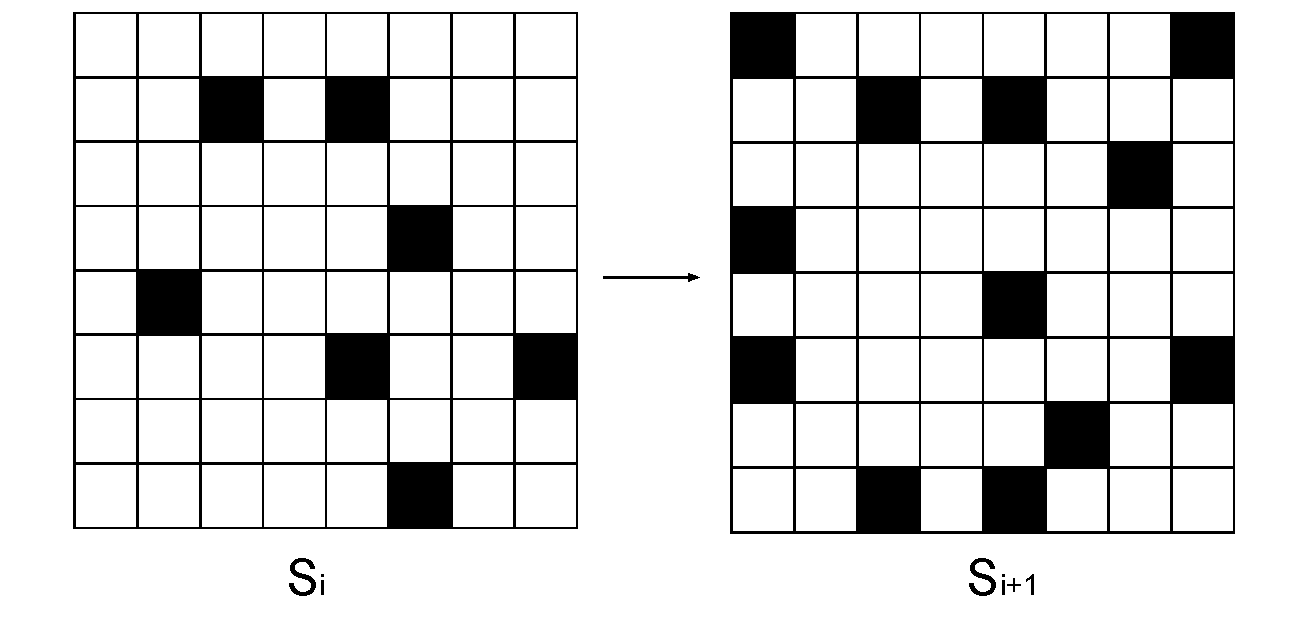
\includegraphics[width=100mm,scale=0.5]{figures/UniverseA1.pdf}
   \caption{Graphical representation of the dynamical change of a universe with
   $n=8$.}
\end{figure} 
\end{myex}

From the assumption \textbf{A1} we can deduce some consequences.
\begin{myclaim}
Any universe that satisfies \textbf{A1} has at least one element that can exist
in more than one substate.
\end{myclaim}

The f of this claim is obvious: an empty set cannot change. A set in which
all elements can exists in only one substate also cannot change. Therefore, the
simplest universe in which \textbf{A1} holds is a universe with only one element
that can exists in two substates, this is, a bit that changes its value
according to a dynamical law.

\subsection{The scientific method}

Now we need to define what is science in this minimal context. First, let's
define what an agent is.

\begin{mydef}
  An agent $A$ is defined as a subset of the universe $U$. $A(\tau)$ is the
  composition of $A$ at the dynamical value $\tau$. The dynamical evolution of
  $A$ is determined by the dynamical evolution of $U$.
\end{mydef}

This is a very broad definition of an agent, since we define them just as
subsets of the universe, so anything can be an agent. We can safely make this
assumption since humans and computers are subsets of the universe. The
definition implies that agents obey the same physical laws than the universe.
Some philosophers would call this implication a materialistic assumption.

\par

Another definition required for science is the definition of measurement or
observation. This definition is particularly delicate in the context of quantum
theory, so we have to be very careful in its definition. 

\begin{mydef}
  An observation $\hat{O}_A$ is defined as the dynamical process in which the
  state of any subset of an agent $A$ gets correlated to the state of another
  subset of $U$, the object $O$, that may or not be disjoint to $A$.  
\end{mydef}

This definition is also very broad, so let's explain it. When we talk about
observations in the context of humans, we usually understand them as information
from an object acquired by our sensorial system, for example by observing with
our visual system a bunch of photons emitted from a source of light. However,
these terms mean nothing in our minimal model so we need to be more specific.
When we see an object, the process, as far as we know, happens because a photon
coming from the object hits some receptors in our retina producing a chain
reaction that triggers an specific state in some part of the brain. In other
words, an specific part of us (the agent $A$) gets correlated to the state of
the object (a subset of $O$ the universe) as a result of the dynamical evolution
of the universe. The dynamical process that gets both states correlated is an
observation.

\begin{myex}
  In this example we are going to see how an observation translate to our simple
  model of universe. With the same universe than in \ref{example1}, we can
  define a new dynamical law that consists on a 1 doing a random walk in a
  bidimensional grid of zeros. Each time an element $a_{jk}$ switches to 1, it
  gets correlated to the rest of the elements of the universe since all of them
  must be zero. In this case, the agent $A$ is the subset of $U$ containing only
  $a_{jk}$ while the object $O$ can be any subset of $U$. We say then that $A$
  has made an observation $\hat{O}_{A}$.
\end{myex}

We need one more definition to define the scientific method. Science is about
making predictions about the physical world, so we need to define what a
prediction is in our minimal context.



\begin{mydef}
  A prediction is... \textit{(I haven't come yet with a successful definition
  for a prediction. I'm trying to formulate it with different agents trying
  to communicate correlations about the "future" of some subsystem of U)}
\end{mydef}

\subsection{Second assumption: Emergency}
\textit{I want to have a formal definition of predictions and the scientific
method before writing this subsection. But it's just a corollary of the
anthropic principle: if we are able to do science, then the dynamical law of the
universe must allow for scientific agents to be generated. For example, a simple
cellular automaton that converges to a stable state wouldn't fulfill this
assumption.}

\chapter{Machine Learning theory} 

TO BE WRITTEN.

\chapter{Experimenter-Analyzer model}

In this section, we are going to present our proposal for a basic model for a
machine learning set-up that designs an experiment applying the scientific
method. It is a model that mixes reinforcement learning and and deep learning to
create agents able to design strategies for experiments, using as feedback only
the quality of the predictions about properties of the physical system made
exclusively from the data the agents collect. 

One of the cornerstones of our model is the principle of modularity: in order to
be applicable to a wide range of set-ups it needs to be constituted by simple
individual elements that can be combined to build complex learning loops. The
agent that will learn to design experiments and make predictions with them is
composed by two different kinds of sub-agents that complement each other:

\begin{itemize}
  \item \textbf{Experimenters}: this kind of sub-agents are reinforcement
  learning based agents. Its goal is to take decisions about influencing the
  dynamics of the physical system (e.g by modifying a parameter of a controlled
  experiment) or about what measurements to make (eg. by choosing what property
  of the physical system to measure). It could be that the choice of
  measurement modifies as well the dynamics of the physical system (eg. by
  choosing which slit to "look at" in the double slit experiment). To choose
  what actions to take they can consider previous observations and other kind of 
  information.
  \item \textbf{Analyzers}: this kind of sub-agents are learning agents
  that take the information gathered by the Experimenters to make predictions
  about the environment. Then, based on the accuracy of those predictions
  compared to the real values \footnote{One may ask how these real values are
  obtained. Those values could be obtained by measurements made by other
  Experimenters that form part of the learning agent. However, for simplicity in
  the work presented here we assume that the real values needed to check the
  validity of the prediction are always accessible with unlimited accuracy to
  the agent. In the context of this modular framework we could assume that we
  have an Experimenter that its only possible action is to measure the real
  value of the target property.} of the environment a reward is generated to
  train all the sub-agents. 

\end{itemize}


\begin{figure}
  \centering
  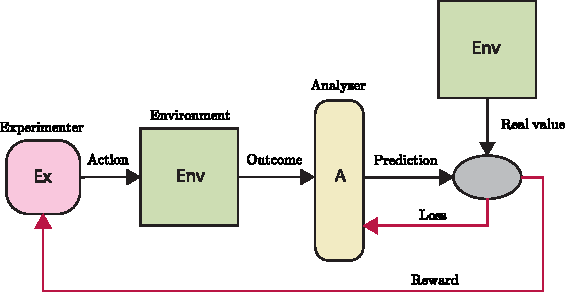
\includegraphics{figures/SimpleSetUp.pdf}
  \caption{Diagram of the simplest combination of elements. The feedback loop
  consists on the following: 1. The Experimenter takes an action. 2. The
  environment gives back an outcome resulting from the action. 3. The action is
  taken by the analyzer and used to make a prediction. 4. The prediction about
  the environment and the real value of the environment are compared to generate
  the loss and the reward to train the Analyzer and the Experimenter.}
  \label{fig:simplesetup}
\end{figure}

To get a better understanding of the purpose of each part of the model let's
take a look to the simplest structure that can be formed with the model (Fig.
\ref{fig:simplesetup}). To illustrate it let's imagine a simple physical set-up.
Suppose we have a simple gravity pendulum of length $L$ and mass $M$ and the
goal is to find the oscillation period on Earth's surface. We know the period is
a function only of the length $L$ and the value of the Earth's gravity (which we
assume to be constant): $T \approx 2\pi\sqrt{\frac{L}{g}}$, so the value of the
mass $M$ is irrelevant for the purpose, but in principle this is unknown to the
agent. In this set-up we give the Experimenter two possible actions to take (but
only one try): either measuring the mass $M$ (eg. by using a calibrated spring)
or measuring the length $L$ of the string (e.g by using a calibrated ruler).
When the Experimenter takes an action over the Environment, it produces an
outcome (either the mass $M$ or the length $L$). This outcome is passed to the
Analyzer which tries to make a guess of the period based on the value of the
outcome of Experimenter's action. Then the real period of the pendulum is
observed and compared to the value predicted by the Analyzer. Depending on the
result of the comparison a loss and a reward are generated to train the
Experimenter and the Analyzer. In general: the closer the value of the
prediction to the actual value the smaller the loss and the higher the reward.
After the iteration is completed, a new pendulum with new values of $M$ and $L$
(ideally generated uniformly at random under the i.i.d. assumption) is generated
and the process starts again.

The goal in the set-up depicted in Fig. \ref{fig:simplesetup} is to form a
feedback loop between the Experimenter and the Analyzer from the, at first
unknown, correlations between the outcomes and the values to be predicted. The
better the Experimenter gets, the better the data available for the Analyzer to
make better predictions that will generate better rewards for the Experimenter.
Hopefully, this feedback loop will converge to an optimal experiment strategy
and an optimal model for the predictions. At the beginning both sub-agents will
start by giving random outputs since they are not trained. This is what we call
the \textit{exploration phase} and it is of fundamental importance for the
feedback loop to start. It can be artificially enforced, for example with
$\epsilon$-greedy algorithms that we will discuss later in this work. If there
exists any correlation between the choices of the Experimenter and the target
value to be predicted, the Analyzer's training algorithm (usually Stochastic
Gradient Descent) can exploit those correlations to start the descent to some
local or global minimum. This working principle is somehow similar to the use of
artificial neural networks for feature selection in classical machine learning
theory.

The alert reader may have noted that in \ref{fig:simplesetup} the Analyzer has
no apparent way of telling which action the Experimenter took, since it only
receives the outcome of the experiment. Therefore the Analyzer doesn't know if
what is receiving is the value of $M$ or $L$. Although it may appear counter
intuitive, the Analyzer doesn't care in this particular set-up. The optimal
strategy is to treat everything as if it were $L$ since knowing the value of $M$
doesn't provide any information about $T$. However, it may make sense for the
Analyzer to know when $M$ is provided if the objective is to minimize the loss
function (e.g. if the Analyzer knew that the value corresponds to $M$ the
optimal prediction would be the random guess that minimizes the loss). In
practice, unless the distributions where $M$ and $L$ are generated from are the
same, the Analyzer learns to differentiate them with high confidence just by
value of the outcome. However, in other set-ups this may not be the case and the
information about what actions were taken is useful for the Analyzer to make the
predictions. In this case, we should also feed the actions as inputs to the
Analyzer. As we will see, these Experiment-Analyzer loops can grow very quickly
in complexity when several sub-agents are involved. This is why we introduce the
concept of \textit{buffer}.

In our model we can use a buffer to store everything that we might want to feed
to the agents. Usually this will be the actions taken and the outcomes obtained
in every observation of the environment, although we have the freedom to add
whatever we might need. It is just a variable to store information. This
variable is not strictly needed, since we could establish directly the
connections between the different subagents and environment outcomes. However,
when we have a few sub-agents with several outcomes it becomes very difficult to
keep track of each connection and to represent them. In these cases, the concept
of buffer becomes highly useful from an illustrative point of view. Usually, the
buffer is emptied at the end of each episode or iteration of the learning loop.
We could not do so, but in practice, keeping the data in the buffer doesn't
provide any easy advantage since to use it we should solve many challenges, for
example an increase on the number of features feeded to the agents each episode.
We won't refer the buffer as \textit{memory} in this work, since the word
\textit{memory} is reserved for an element of some versions of sub-agents that
doesn't restart in each iteration. 


\begin{figure}
  \centering
  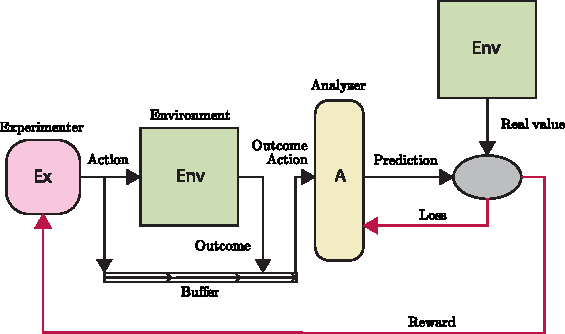
\includegraphics{figures/SimpleSetUp(Buffer).pdf}
  \caption{Diagram of a simple learning loop with buffer. In this case, the
  process is identical to the process depicted in Fig. \ref{fig:simplesetup}
  with the difference that the values of the action and the outcome are stored
  in the buffer, and then passed to the analyzer. In this case the information
  about which action was taken is available to the Analyzer.} 
  \label{fig:simplesetupbuffer}
\end{figure}

\section{General elements and definitions}
In this section let's define more formally some of the elements and concepts of
our model.
\begin{itemize}
    \item \textbf{Simulated physical environment (SPE): } it represents the
    physical world that determines the outcomes of all the measurements realized
    by the agent. It is completely represented by a state $ s \in S $, where $S$
    is the set of all possible states in which the SPE can be. For this
    particular model we assume that the evolution of the system is assumed to be
    given by a Markovian function $f: S \rightarrow S$ such that
    $f(s_\tau)=s_{\tau+1}$. This function maybe deterministic or not.
    \item \textbf{Agent:} the agent is formed by the composition of two kind of
    different subagents:
    \begin{itemize}
        \item \textbf{Experimenter:} this part has the task of making decisions
        that will have an effect on the observations. This effect could be due
        to the influence of the decisions in the evolution of the system (for
        example, if the agent decides to shoot a bullet to a box with a certain
        velocity) or due to the fact that the decisions themselves could be what
        observations to make (for example, choosing to measure the position of a
        box within a spatial range). This agent will be implemented using
        reinforcement learning techniques. Mathematically it can be represented
        by a trainable function $E:\mathcal{X}\rightarrow\mathcal{A}$ where
        $\mathcal{A}$ represents the space of possible actions and $\mathcal{X}$
        is an arbitrary space that can represent any accessible information that
        might be useful to make a choice of action. In the context of
        reinforcement learning, $\mathcal{X}$ is the set of states of the
        sub-agent's environment\footnote{Not to be confused with the SPE.}.
        \item \textbf{Analyzer:} the goal of this part of the agent is to
        process the data collected in the observations after the action of the
        Experimenter to predict a physical property of the SPE. This property
        could be a physical parameter of the system or a prediction of the
        dynamics of the environment. It will usally consist of a regular
        regression neural network or an autoencoder, depending on the specific
        set-up. But we could use any trainable function like SVMs or any kind of
        regression. Mathematically it can be represented by a trainable function
        $ A :\mathcal{M} \rightarrow \mathcal{P}$, where $\mathcal{M}$ is the
        space of measurements and $\mathcal{P}$ is the space of predictions.
  \end{itemize}
    \item \textbf{Orchestration:} when coding we will call Orchestration
    everything that connects the different parts to complete a feedback loop.
    For example, one of the tasks of the Orchestration is to transform the state
    of the SPE into the measurements received by the Analyzer. The Orchestration
    is needed when we simulate fictitious physical situations in a computer to
    test our models. It represents somehow something analogous to the sensors
    and wires that connect the external environment to the processor of an
    autonomous robot.
\end{itemize}

\begin{myex}
Let's complete the example of the pendulum to fully illustrate the architecture.
First, we define the SPE. Let's assume that the mass of the pendulum and the
length of the string are sampled uniformly at random from the intervals \break
$0.1$ kg $< M < 1$ kg and $ 0.1$ m $<L<1 $ m. The space of states of the SPE
is then:
 \begin{equation}
  S\equiv \{(m,l):m \in \left[0.1, 1\right],l \in [0.1,1]\}
 \end{equation}
Now, let's define an Experimenter. In this case, the Experimenter's environment
space $\mathcal{X}$ is the empty set $\emptyset$, since there is no input. This
means that the agent takes the action based solely on the rewards obtained. The
action space $\mathcal{A}$ is just $\{0,1\}$, with 0 representing the action of
measuring the mass and 1 the action of measuring the length.

We can therefore set a very basic decision rule for our Experimenter agent:

\begin{itemize}
  \item Let $\textbf{Q}=(q_0,q_1)$ be the value table, where $q_0$ and $q_1$ are
  the values associated with the actions 0 and 1 respectively.  $Q$ can be also
  understood as a trainable function $Q:\mathcal{X}\times\mathcal{A} \rightarrow
  \mathbb{R}$. Initially $Q(a)=0 \; \forall a \in \mathcal{A}$. 
  \item  Every episode, the agent takes an action $a$ and receives a reward $r$
  after taking the action.
  The update rule for $\textbf{Q}$ is the following:
  \begin{equation}
    q_a\leftarrow q_a + r
    \label{update_rule1}
  \end{equation}
  This is, the value $q_a$ is just the cumulative reward obtained by the 
  action $a$. 
  \item The agent's policy $E:\emptyset  \rightarrow \mathcal{A}$ or 
  decision rule is:
  \begin{equation}
    a = \argmax_{x \in \mathcal{A}} Q(x)
    \label{argmax_policy}
  \end{equation}
  This is, the Experimenter takes the action $a$ with the highest $q_a$, and 
  $E$ is trained by updating $\textbf{Q}$ each episode.
\end{itemize}

Note that the choice of \eqref{update_rule1} is just to illustrate that we can
build Reinforcement Learning agents with very simple rules. We could have
chosen instead of the cumulative reward the average reward obtained with the 
action, but the working principle would be identical.

However, our policy is still flawed, since the first action that gets a reward
would always be elected afterward independently of its optimality. To solve this
we can force the agent to initially explore different options ignoring the
decision rule, and slowly, when the values $q_a$ are more reliable, let the
agent choose according to \eqref{argmax_policy}. The easiest way to achieve that
is with an $\epsilon$-greedy decision algorithm: we set an exploration rate
$\epsilon$ that decreases in each episode until it reaches a minimum value
$\epsilon_\text{min}\geq 0$. The Experimenter is set to take the
\eqref{argmax_policy} policy with probability of $P_{\text{greedy}}=1-\epsilon$
and a random action with a probability of $P_{\text{random}}=\epsilon$. We have
the freedom to choose how to decrease the value of $\epsilon$, and it may have a
crucial impact on the training. A very popular rule is to decrease the value
constantly by subtracting $\delta_\epsilon = 1/N$, where $N$ is the number
iterations of the training. So in each episode:
\begin{align}
  &\text{if}\; \; \epsilon > \epsilon_\text{min} \;\;\; &\epsilon&\leftarrow\epsilon - \delta_\epsilon \\
  &\text{else} \; \;  &\epsilon &\leftarrow \epsilon_\text{min}
\end{align} 


For the Analyzer, we set a trainable real function $A: S \rightarrow
\mathbb{R}$. We can use any trainable function, but to keep it simple let's use
a regular feed-forward neural network with one hidden layer of two neurons,
trained with the Stochastic Gradient Descent (SGD) algorithm and a the Mean
Squared Error (MSE) loss.

We need now to define how to calculate the reward.  In our case we want the
reward function to be high when the Analyzer predicts a period $T_\text{pred}$
close to the real period of the pendulum and low when the period prediction is
far. So, ideally we would like a function that:
\begin{align}
       r(T_{\text{pred}} \approx T) &\approx 1\\
       r(T_{\text{pred}}>> T \text{ or } T_{\text{pred}} << T) & \approx 0
\end{align}
One natural way to achieve this is using a Gaussian distribution over the
relative error $\Delta=(T-T_{\text{pred}})/T$. This is:
\begin{equation}
   r(\Delta)=\exp\left(-\frac{1}{2}\left( \frac{\Delta}{\sigma} \right) ^2\right)
\end{equation}
and $\sigma$ allows us to modify the precision we want in order to achieve a 
reward.

Now we have every element defined. Let's outline the full algorithm in 
pseudocode:

  \makeatletter
  \def\BState{\State\hskip-\ALG@thistlm}
  \makeatother
  \begin{algorithm}
    \caption{Simple learning loop}\label{pendulum}
    \begin{algorithmic}[1]
    \Procedure{Pendulum}{}
    \BState count = 0
    \BState $\textbf{while } \text{count} < N:$
    \State $ M, L \gets \text{random sample }  M, L$
    \State $ T \gets T(L)$
    \State $ \text{pendulum} \gets [M,L,T]$
    \State $ \text{action} \gets \argmax Q $
    \State $ \text{measurement} \gets \text{pendulum[action]}$
    \State $ \text{prediction} \gets \text{analyzer(measurement)}$
    \State $ \text{Apply SGD to Analyzer with data point } (\text{measurement},T)$
    \State $ \text{reward} \gets \text{reward}(\text{prediction}, T)$
    \State $ Q[\text{action}] \gets Q[\text{action}]+ \text{reward}$ 
    \State $ \text{count }\gets \text{count} + 1$
    \EndProcedure
    \end{algorithmic}
    \end{algorithm}
\end{myex}

Let's see how this simple algorithm performs in the task. Ideally, the
Experimenter would find the optimal policy which consists in choosing always to
measure the length and the Analyzer would learn to estimate accurately $T$ from
the data obtained by the Experimenter. In our experiments, with this simple
structure of only two neurons and the very naive reinforcement learning policy
the agent consistently finds the optimal action (to measure $L$). It also
accurately predicts the value of $T$ in less than 10,000 episodes. With less
episodes it is less consistent in finding the optimal policy.

\begin{figure}[h]
  \centering
  \begin{subfigure}{.5\textwidth}
    \centering
    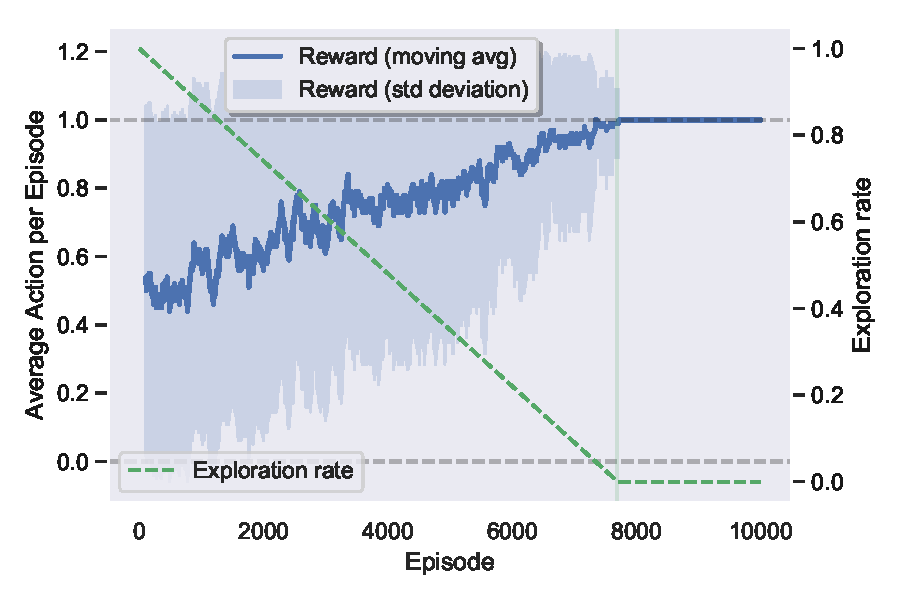
\includegraphics[width=1\linewidth]{figures/Avg-Action-Pendulum.pdf}
    \caption{Moving average of the actions}
    \label{fig:ActionAveragePendulum}
  \end{subfigure}%
  \begin{subfigure}{.5\textwidth}
    \centering
    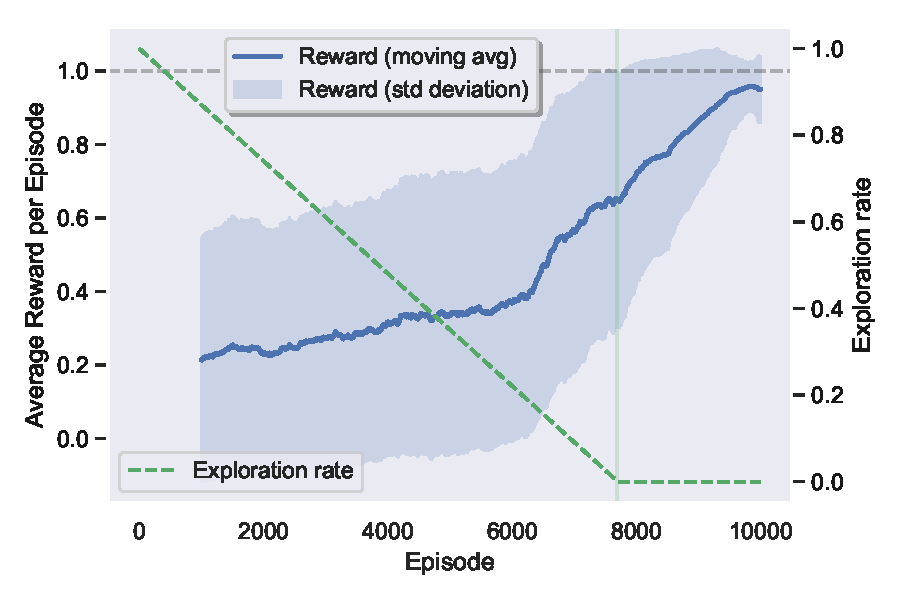
\includegraphics[width=1\linewidth]{figures/Reward-Pendulum.pdf}
    \caption{Moving average of the reward}
    \label{fig:RewardAveragePendulum}
  \end{subfigure}


  \caption{(a) The moving average of the actions taken in each episode. We can
  see how it starts taking both actions evenly with an average of 0.5. This is
  expected since at the beginning $\epsilon \approx 1$. As $\epsilon$ decreases
  the Experimenter starts to take more greedy actions and gets biased towards
  the action 1 (measure $L$). This bias appears as a result of the existing
  correlation between $L$ and $T$, but not between $M$ and $T$. This correlation
  is exploited by the SGD algorithm for the neural network of the Analyzer. (b)
  The moving average of the reward obtained in each episode. At the beginning
  the reward obtained is low and similar to those obtained with random guesses.
  However, it increases slowly, apparently because the Analyzer starts to
  exploit slightly the correlation between $L$ and $T$. This slight improvement
  over the prediction for the outcomes of Action 1, creates the bias that starts
  the feedback loop. Values: $\sigma=0.05$, $N=10000$,
  $\text{lr}_\text{Analyzer}=0.01$, Optimizer = Adam}
  \label{fig:PendulumTraining}
  \end{figure}

  In the figures Fig. \ref{fig:PendulumTraining} and Fig.
  \ref{fig:PendulumError} we can observe the evolution of different parameters
  during the training. All the parameters show successful learning of both, the
  optimal policy and the prediction of the period. More complex neural network
  structures and longer trainings can achieve much lower errors. However, this
  is not a surprise since once the optimal policy is obtained the process just
  consists on fitting a continuous single variable function. A task that can be
  solved optimally by a single layered sigmoidal neural network
  \cite{cybenko1989approximation}. This pendulum example, although trivial, is
  useful to appreciate the working principle behind the Experimenter-Analyzer
  architecture and how the feedback loop is formed. In the next section we are
  going to explore less trivial examples with more complex learning loops.

  
\begin{figure}[t]
  \centering
  \begin{subfigure}{.5\textwidth}
    \centering
    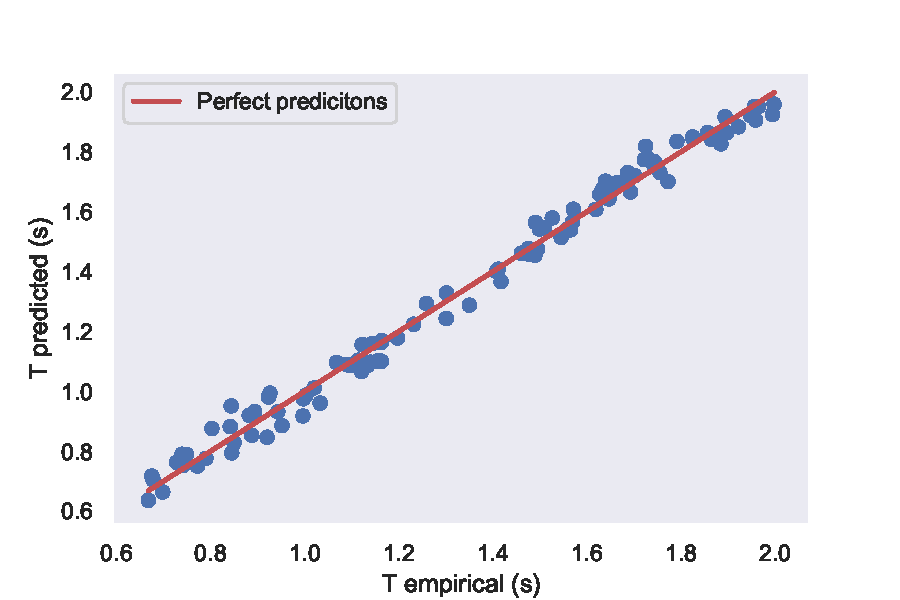
\includegraphics[width=1\linewidth]{figures/Real-vs-Pred-Pendulum.pdf}
    \caption{Real T vs Predicted T}
    \label{fig:RealvsPredictedPendulum}
  \end{subfigure}%
  \begin{subfigure}{.5\textwidth}
    \centering
    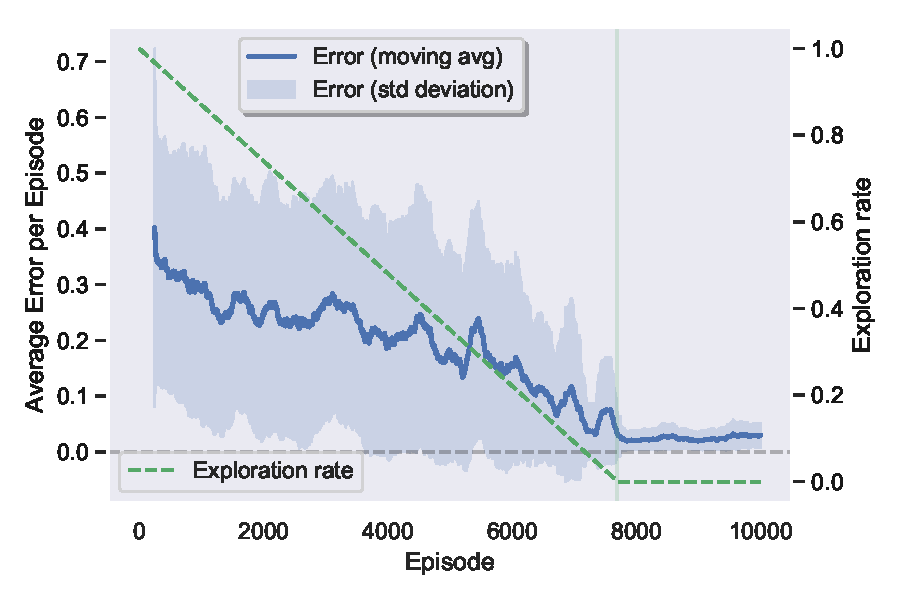
\includegraphics[width=1\linewidth]{figures/Error-Pendulum.pdf}
    \caption{Moving average of the error}
    \label{fig:ErrorAveragePendulum}
  \end{subfigure}
  \caption{(a) A sample of the predictions made by trained agent. We can see
  how it fits the $y=x$ line, showing that it learned the relation between
  $L$ an $T$. (b) In this figure we can see how the error decreases to almost 
  zero with very low deviation.Values: $\sigma=0.05$, $N=10000$,
  $\text{lr}_\text{Analyzer}=0.01$, Optimizer = Adam
  }
  \label{fig:PendulumError}
  \end{figure}

\chapter{E-A architecture in different scenarios} 
\label{Scenarios}
\section{Scenario 1: Modified multi-armed bandit}
In the first section of this chapter we are going to study a modified version of
the classical Multi-armed bandit problem, a classical problem of Reinforcement 
Learning and Probablity Theory. We will show that we can map any experiment 
consisting of a non-interactive discrete choice measurements to our modified
multi-armed bandit. 

\subsection{General multi-armed bandit problem}

Suppose that we have an agent that has access to a k-armed bandit. Each time the agent pulls
one of the $k$ levers the bandit produces a reward. The objective
of the agent is to maximize the obtained reward in a determined number of 
trials or episodes $N$, but the agent doesn't know how the bandit produces 
the rewards. Its only way of getting information about the reward system is 
by trial and error by pulling the levers and obtaining rewards.

Mathematically we can model our agent as an Experimenter 
$E:\mathcal{X}\rightarrow\mathcal{A}$, where the action space is 
$\mathcal{A}=\{0,1,...,k\}$ and the state space $\mathcal{X}$ is again the 
empty set $\emptyset$. The bandit can be modelled as a probabilistic
function $R:A\times ... \rightarrow \mathbb{R}$, with "$...$" meaning that
in principle the generated reward can depend on anything, for example, the
previous actions, the previous rewards, the number of trials, the number
of times a lever has been pulled, etc. This is an extremely general problem,
so often authors make assumptions on $R$. For example, $R$ being Markovian if
depends only on the last rewards and/or actions. Or stationary if 
$R$ can be modeled as a set of immutable distributions $R=\{R_1,... , R_k\}$, 
each distribution being associated with the rewards delivered by each of the 
arms of the bandit.

We define the value $Q^*(a)=q^*_a$ of an action $a \in \mathcal{A}$ as the true
expected or mean reward associated to the action. We denote by $a_n$ the action
taken in the $n^\text{th}$ episode, and $r_n$ the reward obtained. This is:
\begin{equation}
  Q^*(a) = \mathbb{E}[r_n|a_n = a]
\end{equation}
Note that, although we don't write it explicitly, $Q^*(a)$ can also depend on 
any of the subsets of the domain of $R$.
The optimal strategy for the k-armed bandit problem is to always choose 
$a*=\argmax Q^*(x)$.

Most reinforcement learning approaches to this problem look for an estimate of
$Q^*(a)$, $Q(a)$, and base their choice on $a=\argmax Q(x)$. In general, the
best algorithm depends deeply on the characteristics of $R$, e.g., an algorithm
that works well for stationary bandits can perform very poorly on non-stationary
bandits. The interested reader can read a gentle introduction to the multi armed
bandit problem in the Chapter 2 of \cite{sutton2018reinforcement}. We are not
going to discuss here many of the approaches to solve the mult-armed bandit
problem. However, let us outline a very simple algorithm that works particularly
well for non-stationary bandits. 

\subsection{Simple Reinforcement Learning algorithm for nonstationary
multi-armed bandit}

Let us outline a simple algorithm that we will use later in this section. This
algorithm can be understood as a particular case of the Q-Learning algorithm,
where the state space of the experimenter $\mathcal{X}$ is the empty set
$\emptyset$ and the discount factor $\gamma$ is set to zero. The update rule for
the estimate $Q(a)$ each time the action $a$ is taken is:

\begin{equation}
  Q(a) \leftarrow Q(a) + \alpha \left( r - Q(a) \right)
  \label{simpleQ}
\end{equation}

where $\alpha \in (0,1]$ is the called the learning rate, $Q_{a}$ is the
estimate value for the action $a$ and $r$ is the reward obtained after taking
the action $a$.

If we name by $Q_n$ the estimate of $Q^*(a)$ for an arbitrary action $a$ at the
 $(n)^\text{th}$ time the action $a$ was taken, then due to \eqref{simpleQ} we
 have that:

 \begin{align}
  Q_{n+1} &=Q_{n}+\alpha\left(r_{n}-Q_{n}\right) \\
  &=\alpha r_{n}+(1-\alpha) Q_{n} \\
  &=\alpha r_{n}+(1-\alpha)\left[\alpha r_{n-1}+(1-\alpha) Q_{n-1}\right] \\
  &=\alpha r_{n}+(1-\alpha) \alpha r_{n-1}+(1-\alpha)^{2} Q_{n-1} \\
  &=(1-\alpha)^{n} Q_{1}+\sum_{i=1}^{n} \alpha(1-\alpha)^{n-i} r_{i}
  \label{weighted_sum}
  \end{align}
The last equation, \eqref{weighted_sum}, is just a weighted average of the
rewards obtained, where the weights give exponentially less importance to 
rewards coming from distant actions in the past. Sometimes is known as \textit{
  exponential recency-weighted average}.

\begin{myclaim}
  If $\alpha$ is constant on $n$, the exponential recency-weighted average is
  also a convex sum of the rewards obtained.\\
\end{myclaim}
  \textit{f:} Since $\alpha \in (0,1]$ all the coefficients are no greater
  than 1. We just need to prove that $\forall n$ they sum to one. If we write 
  the sum $S_n$ of the coefficients at the time $n$:
  \begin{equation}
    S_n=(1-\alpha)^{n} + \sum_{i=1}^{n} \alpha(1-\alpha)^{n-i}
    \label{eq:sum}
  \end{equation}
  We also have that: 
  \begin{align}
    (1-\alpha)^n &= (1-\alpha)(1-\alpha)^{n-1} \\
    &=(1-\alpha)^{n-1}-\alpha(1-\alpha)^{n-1}
    \label{eq:aux}
  \end{align}
  Inserting \eqref{eq:aux} in \eqref{eq:sum} we get:
  \begin{align}
    S_n&=(1-\alpha)^{n-1}-\alpha(1-\alpha)^{n-1}+\sum_{i=1}^{n} \alpha(1-\alpha)^{n-i}\\
    &=(1-\alpha)^{n-1} + \alpha \sum_{i=1}^{n-1} \alpha(1-\alpha)^{n-1-i}
  \end{align}
  If we call $l=n-1$ we obtain exactly \eqref{eq:sum} but with $l$ instead of 
  $n$. We can repeat this process until the new index happens to be $1$. Then
  we have:
  \begin{equation}
  S_n = (1-\alpha) + \alpha = 1 \qed 
\end{equation}

Lets outline with pseudo-code how this agent would work:

\makeatletter
\def\BState{\State\hskip-\ALG@thistlm}
\makeatother
\begin{algorithm}
  \caption{}\label{Non-stationary multiarmed-bandit}
  \begin{algorithmic}[1]
  \Procedure{Non-stationary multiarmed-bandit agent}{} \BState count = 0 \BState
  $\textbf{while } \text{count} < N:$ \State action $\gets$ $\argmax Q$ \State
  reward $\gets$ bandit(action) \State Q[action] $\gets$ Q[action] + $\alpha$
  (reward - Q[action]) \State count $\gets$ count + 1 \EndProcedure
  \end{algorithmic}
  \end{algorithm}

  If we pay attention to the pseudo-code we see that for taking the first action
  we must have an initial estimate $Q_1$ for each action. These initial
  estimates aren't irrelevant. They play an important role in the convergence of
  the algorithm. For example, if we set $Q_1=0 \; \; \forall a \in \mathcal{A}$,
  the $\argmax Q_1$ will output a random action. Therefore, the training can be
  biased towards that action depending on the initial reward. Sometimes a good
  strategy is to set high values of $Q_1$ for all actions. This will make the
  agent overoptimistic in the estimate, forcing it to explore all options until
  getting a more realistic estimate of the reward.

  It can be shown that choosing the following learning rate give us an
  exponential recency-weighted average without initial bias:
  \begin{equation}
    \alpha_n = \beta/o_n
  \end{equation}
  where $\beta$ is a constant parameter and $o_n$ is a constant step size
  updating parameter so that:
  \begin{equation}
    o \gets o + \beta(1-o) 
  \end{equation}
  with an initial value of $o_1=0$ for all actions.


  
\section{Scenario 2: Spring-Shooting experiment}

\section{Scenario 3: Shooting with two position sensors}

So far we have used always the same architecture with a Q-table that chooses
a predefined experimenter to optimize the reward obtained by the Analyzers 
prediction. However, it may be the case in which we have experiments with 
several measurements or actions that depends on the outcomes of the previous
observations.

\clearpage
%
%
%%%%%%%%%%%%%%%%%%%%%%%%%%%%%%%%%%%%%%%%%%%%%%%%%%%%%%%%%%%%%%%%%%
%%%%%%%%%%%%%%%%%%%%%%%%%%%%%%%%%%%%%%%%%%%%%%%%%%%%%%%%%%%%%%%%%%
%% APPENDIX
%%%%%%%%%%%%%%%%%%%%%%%%%%%%%%%%%%%%%%%%%%%%%%%%%%%%%%%%%%%%%%%%%%
%%%%%%%%%%%%%%%%%%%%%%%%%%%%%%%%%%%%%%%%%%%%%%%%%%%%%%%%%%%%%%%%%%
%







\begin{appendix}
%
%%%%%%%%%%%%%%%%%%%%%%%%%%%%%%%%%%%%%%%%%%%%%%%%%%%%%%%%%%%%%%%%%%
%% HEADER APPENDIX
%%%%%%%%%%%%%%%%%%%%%%%%%%%%%%%%%%%%%%%%%%%%%%%%%%%%%%%%%%%%%%%%%%
%






\lhead[\fancyplain{\scshape Appendix \thechapter}
{\scshape Appendix \thechapter}]
{\fancyplain{\scshape \leftmark}
  {\rightmark}}
%
\rhead[\fancyplain{\scshape \leftmark}
{\scshape \leftmark}]
{\fancyplain{\scshape Appendix \thechapter}
  {\scshape Appendix \thechapter}}
%




%%%%%%%%%%%%%%%%%%%%%%%%%%%%%%%%%%%%%%%%%%%%%%%%%%%%%%%%%%%%%%%%%%
%% CHAPTERS APPENDIX
%%%%%%%%%%%%%%%%%%%%%%%%%%%%%%%%%%%%%%%%%%%%%%%%%%%%%%%%%%%%%%%%%%
%
%\include{f}






\chapter{Appendix ?} \label{app:pgm}

\blindtext







%
%
%\include{derivations}
% \chapter{Another Chapter in the Appendix}
% \label{cha:anotherchapterintheappendix}
% 
% Each chapter of the appendix is better included by the command 
% \emph{$\backslash$include\{file\}}.
% %



\clearpage
%
%%%%%%%%%%%%%%%%%%%%%%%%%%%%%%%%%%%%%%%%%%%%%%%%%%%%%%%%%%%%%%%%%%
%% HEADER BIBLIOGRAPHY
%%%%%%%%%%%%%%%%%%%%%%%%%%%%%%%%%%%%%%%%%%%%%%%%%%%%%%%%%%%%%%%%%%
%
\lhead[\fancyplain{\scshape Appendix}
{\scshape Appendix}]
{\fancyplain{\scshape \leftmark}
  {\scshape \leftmark}}
%
\rhead[\fancyplain{\scshape \leftmark}
{\scshape \leftmark}]
{\fancyplain{\scshape Appendix}
  {\scshape Appendix}}
  
  
  
  
  
  
  
  %%%%%%%%%%%%%%%%%%%%%%%%%%%%%%%%%%%%%%%%%%%%%%%%%%%%%%%%%%%%%%%%%%
%% LIST OF FIGURES
%%%%%%%%%%%%%%%%%%%%%%%%%%%%%%%%%%%%%%%%%%%%%%%%%%%%%%%%%%%%%%%%%%
% \addcontentsline{toc}{chapter}{\numberline{}List of Figures}
% \listoffigures
%\clearpage
%
%%%%%%%%%%%%%%%%%%%%%%%%%%%%%%%%%%%%%%%%%%%%%%%%%%%%%%%%%%%%%%%%%%
%% LIST OF TABLES
%%%%%%%%%%%%%%%%%%%%%%%%%%%%%%%%%%%%%%%%%%%%%%%%%%%%%%%%%%%%%%%%%%
% \addcontentsline{toc}{chapter}{\numberline{}List of Tables}
% \listoftables
%\clearpage
%


%
%%%%%%%%%%%%%%%%%%%%%%%%%%%%%%%%%%%%%%%%%%%%%%%%%%%%%%%%%%%%%%%%%%
%% BIBLIOGRAPHY
%%%%%%%%%%%%%%%%%%%%%%%%%%%%%%%%%%%%%%%%%%%%%%%%%%%%%%%%%%%%%%%%%%
\bibliographystyle{plain}
\bibliography{references}
%%%%%%%%%%%%%%%%%%%%%%%%%%%%%%%%%%%%%%%%%%%%%%%%%%%%%%%%%%%%%%%%%%
%% END OF APPENDIX
%%%%%%%%%%%%%%%%%%%%%%%%%%%%%%%%%%%%%%%%%%%%%%%%%%%%%%%%%%%%%%%%%%
%
\end{appendix}
%
%%%%%%%%%%%%%%%%%%%%%%%%%%%%%%%%%%%%%%%%%%%%%%%%%%%%%%%%%%%%%%%%%%
%% INDEX
%%%%%%%%%%%%%%%%%%%%%%%%%%%%%%%%%%%%%%%%%%%%%%%%%%%%%%%%%%%%%%%%%%
%
%\printindex
%
%%%%%%%%%%%%%%%%%%%%%%%%%%%%%%%%%%%%%%%%%%%%%%%%%%%%%%%%%%%%%%%%%%
%% END FRAME
%%%%%%%%%%%%%%%%%%%%%%%%%%%%%%%%%%%%%%%%%%%%%%%%%%%%%%%%%%%%%%%%%%
%
\end{document}
%
%%%%%%%%%%%%%%%%%%%%%%%%%%%%%%%%%%%%%%%%%%%%%%%%%%%%%%%%%%%%%%%%%%
%%%%%%%%%%%%%%%%%%%%%%%%%%%%%%%%%%%%%%%%%%%%%%%%%%%%%%%%%%%%%%%%%%
%%%%%%%%%%%%%%%%%%%%%%%%%%%%%%%%%%%%%%%%%%%%%%%%%%%%%%%%%%%%%%%%%%
